\chapter{Mengenal Kecerdasan Buatan dan Scikit-Learn}
Buku umum yang digunakan adalah \cite{russell2016artificial} dan  
untuk sebelum UTS menggunakan buku \textit{Python Artificial Intelligence Projects for Beginners}\cite{eckroth2018python}.
Dengan praktek menggunakan python 3 dan editor anaconda dan library python scikit-learn.
Tujuan pembelajaran pada pertemuan pertama antara lain:
\begin{enumerate}
\item
Mengerti definisi kecerdasan buatan, sejarah kecerdasan buatan, perkembangan dan penggunaan di perusahaan
\item
Memahami cara instalasi dan pemakaian sci-kit learn
\item
Memahami cara penggunaan variabel explorer di spyder
\end{enumerate}
Tugas dengan cara dikumpulkan dengan pull request ke github dengan menggunakan latex pada repo yang dibuat oleh asisten riset.

\section{Teori}
Praktek teori penunjang yang dikerjakan :
\begin{enumerate}
\item
Buat Resume Definisi, Sejarah dan perkembangan Kecerdasan Buatan, dengan bahasa yang mudah dipahami dan dimengerti. Buatan sendiri bebas plagiat[hari ke 1](10)
\item
Buat Resume mengenai definisi supervised learning, klasifikasi, regresi dan unsupervised learning. Data set, training set dan testing set.[hari ke 1](10)
\end{enumerate}

\section{Instalasi}
Membuka https://scikit-learn.org/stable/tutorial/basic/tutorial.html. Dengan menggunakan bahasa yang mudah dimengerti dan bebas plagiat. 
Dan wajib skrinsut dari komputer sendiri.
\begin{enumerate}
\item
Instalasi library scikit dari anaconda, mencoba kompilasi dan uji coba ambil contoh kode dan lihat variabel explorer[hari ke 1](10)
\item
Mencoba Loading an example dataset, menjelaskan maksud dari tulisan tersebut dan mengartikan per baris[hari ke 1](10)
\item
Mencoba Learning and predicting, menjelaskan maksud dari tulisan tersebut dan mengartikan per baris[hari ke 2](10)
\item
mencoba Model persistence, menjelaskan maksud dari tulisan tersebut dan mengartikan per baris[hari ke 2](10)
\item 
Mencoba Conventions, menjelaskan maksud dari tulisan tersebut dan mengartikan per baris[hari ke 2](10)
\end{enumerate}


\section{Penanganan Error}
Dari percobaan yang dilakukan di atas, apabila mendapatkan error maka:

\begin{enumerate}
	\item
	skrinsut error[hari ke 2](10)
	\item
Tuliskan kode eror dan jenis errornya [hari ke 2](10)
	\item
Solusi pemecahan masalah error tersebut[hari ke 2](10)

\end{enumerate}

\section{Andri Fajar Sunandhar /1164065}
\subsection{TEORI}
\begin {enumerate}
\item
Definisi, Sejarah dan Perkembangan AI.
\subitem
Kecerdasan buatan merupakan sebuah bidang dalam ilmu computer yang begitu penting di zaman ini dan masa yang akan datang guna mewujudkan sebuah sistem computer yang begitu cerdas. Kecerdasan buatan sudah berkembang begitu pesat dalam 20 tahun terakhir seiring dengan adanya kebutuhan perangkat yang cerdas pada bidang industry dan rumah tangga.
\subitem
Artificial Intelligence atau biasa di singkat dengan AI berasal dari bahasa latin yang dimana intelligence berarti saya paham. AI dimulai dari kemunculan sebuah komputer pada tahun 1940-an, akan tetapi perkembangannya dapat dilacak pada zaman Mesir Kuno. Dalam masa ini dimana perhatian difokuskan dengan kemampuan komputer dalam mengerjakan sesuatu yang dapat dilakukan oleh manusia sehingga kompute tersebut dapat meniru kemampuan dan prilaku manusia secara cerdas.
\subitem
Pada tahun 1955, Newell dan juga Simon telah mengembangkan The Logic Theorist, yaitu program AI pertama. Dimana program tersebut mempresentasikan sebuah masalah sebagai model pohon, lalu diselesaikan dengaan cara memilih cabang yang akan mewujudkan kesimpulan terbenar dan tepat. Program AI tersebut berdampak sangat besar dan dapat mendaji batu loncatan yang cukup penting dalam mengembangkan bidang AI. Sekitar tahun 1956 dimana orang yang dianggap sebagai bapak AI yaitu John McCarthy telah menyelenggarakan konferensi guna menarik para ahli dibidang komputer untuk bertemu, dengan acara yang diberi nama The Dartmouth Summer Research Project On Artificial Intelligence. Dalam konferensi tersebut telah mempertemukan pendiri dan pengembang AI. Pada konferensi tersebut bapak AI John McCarthy mengusulkan definisi AI yaitu merupakan cabang dari sebuah ilmu komputer yang dapat berfokus terhadap pengembangan computer sehingga dapat memiliki kemampuan dan juga prilaku seperti manusia.\cite{ baraja2008kecerdasan}

\item
supervised learning, klasifikasi, regresi dan unsupervised learning. Data set, training set dan testing set.
\subitem
Supervised Learning merupakan sebuah pendekatan yang dimana terdapat data dan variable yang telah ditargetkan sehingga pendekatan tersebut bertujuan untuk mengelompokkan sebuah data ke data yang sudah ada, beda dengan Unsupervised learning yang tidak mempunyai data, sehingga data yang ada harus di kelompokkan menjadi beberapa bagian.
\subitem
Klasifikasi merupakan sebuah kegiatan penggolongan atau pengelompokkan. Menurut kamus besar bahasa Indonesia yang dimana klasifikasi merupakan penyusunan sistem di dalam kelompok atau golongan berdasarkan kaidah atau standar yang telah ditetapkan. Regresi merupakan sebuah metode analisis statistic yang akan digunakan untuk melihat pengaruh variable.
\subitem
Dataset merupakan sebuah objek yang akan mempresentasikan sebuah data dan relasinya di memory. Struktur pada dataset ini mirip dengan data yang ada di dalam database. Training set merupakan bagian dari dataset yang berperan dalam membuat prediksi atau algoritma sesuai tujuan masing – masing. Testing set merupakan bagian dari dataset yang akan di tes guna melihat keakuratatan atau ketepatan datanya.
\end {enumerate}

\subsection{INSTALASI}
Instalasi library scikit dari anaconda, mencoba kompilasi contoh kode dan lihat variable explorer.
\begin {enumerate}
\par
\item Install Aplikasi anaconda
\item buka cmd, lalu install library scikit. ketikan perintah conda install scikit-learn 
\par
\begin{figure}[ht]
\centering
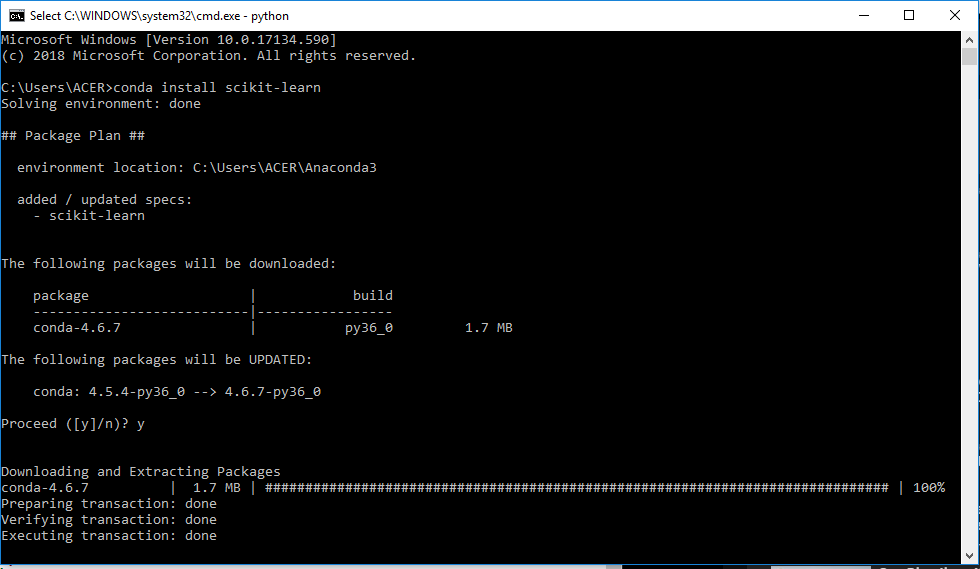
\includegraphics[scale=0.5]{figures/1.png}
\caption{Install library scikit}
\label{contoh}
\end{figure}
\par

\item cek version anaconda dan python
\par
\begin{figure}[ht]
\centering
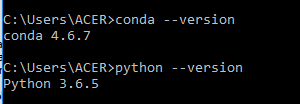
\includegraphics[scale=0.7]{figures/2.png}
\caption{version anaconda dan python}
\label{contoh}
\end{figure}
\par

\item update library scikit dengan perintah pip install -U scikit-learn
\par
\begin{figure}[ht]
\centering
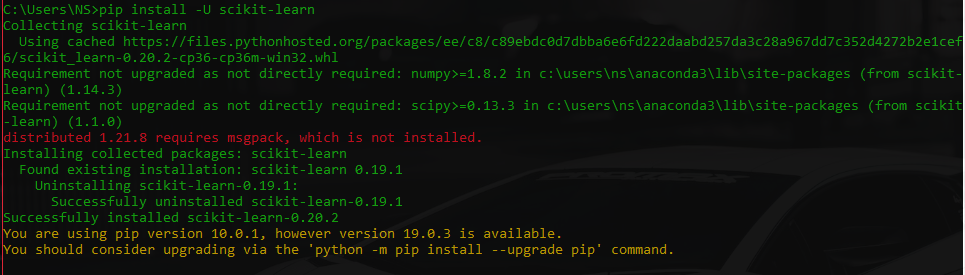
\includegraphics[scale=0.5]{figures/3.png}
\caption{update library scikit}
\label{contoh}
\end{figure}
\par

\item test compile
\par
\begin{figure}[ht]
\centering
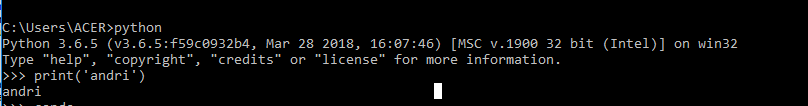
\includegraphics[scale=0.5]{figures/4.png}
\caption{test compile}
\label{contoh}
\end{figure}
\end {enumerate}
\par

Mencoba Loading an example dataset
\begin {enumerate}
\par
\item Dari skalearn menginport dataset kemudian dataset nge load dari iris dan digits
\par
\begin{figure}[ht]
\centering
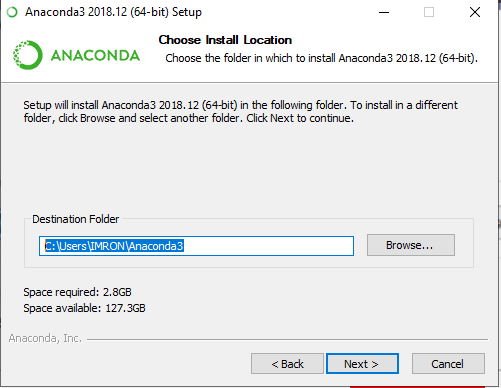
\includegraphics[scale=0.5]{figures/5.png}
\caption{import dataset}
\label{contoh}
\end{figure}
\par
\item mencoba menampilkan data digits
\par
\begin{figure}[ht]
\centering
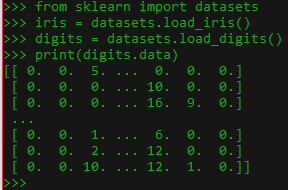
\includegraphics[scale=0.5]{figures/6.png}
\caption{data digits}
\label{contoh}
\end{figure}
\end {enumerate}

